\chapter{Methodology}
\label{chap:methodology}

Choosing which Software Development Life Cycle (SDLC) methodology was a key decision at the beginning of the project; the methodology influences the route that development took during the project's lifetime. The Iterative Development Model has been chosen alongside the use of other key project management methods in other team-focused methodologies, such as Agile \see{chap:pm}.

\section{An Iterative Development Methodology}
\label{methodology:chosen}

There was an initial dissonance when deciding between the Iterative and Incremental models. They are similar, but the Incremental model delivers a portion of the software at a time \see{fig:incremental}, whereas the Iterative model delivers the entire software at the end of each iteration \see{fig:iterative}. Throughout development, there was an ongoing debate as to which model was being used. After reflecting on the project's development, it was clear that the Iterative model was used, despite initially believing that the Incremental model was being implemented. 

\begin{figure}
    \centering
    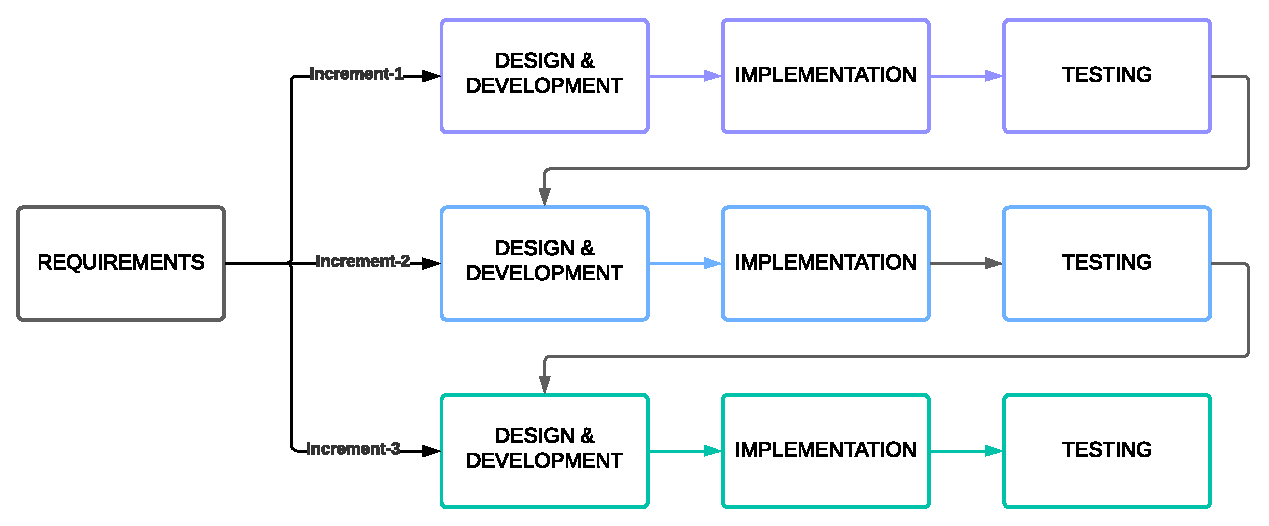
\includegraphics[width=400px]{figures/incremental-model.pdf}
    \caption{Incremental Development Model}
    \label{fig:incremental}
\end{figure}

\begin{figure}
    \centering
    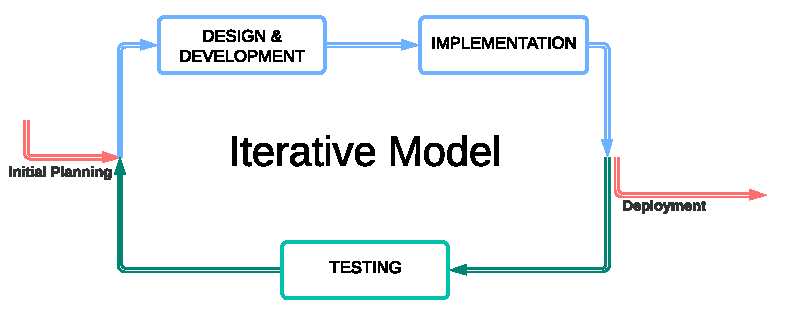
\includegraphics[width=400px]{figures/iterative-model.pdf}
    \caption{Iterative Development Model}
    \label{fig:iterative}
\end{figure}

Once it was understood that the iterative model was used, it was clear that the project's development was more flexible than initially thought. All aspects of the system were improved upon within each iteration, ensuring that the user requirements were met. The model's flexibility to accommodate requirement changes proved fundamental when the initial requirement drafts were updated after research was conducted \see{chap:litrev}. When these requirement changes occurred, new system requirements (SR) were created after breaking down the user stories, and each SR acted as a sub-task \see{chap:requirements}. Each sub-task was given a deadline to ensure changes were made within the iteration. Kanban boards were used to track the progress of all tasks \see{pm:kanban}.

The model was used for this project since the Waterfall Model cannot precisely and completely describe the real software development life cycle (\cite{dapeng_liu_case_2011}). Each iteration represents a full software life cycle vaguely following the waterfall methodology's structure: Requirements analysis, Design, Development, Testing, and Release.

One key downside of the iterative model is when changes are merged between iterations. This introduces a potential discontinuity of design purpose where the user interface and programming interfaces become discontinuous between iterations (\cite{dapeng_liu_case_2011}). To mitigate this, a consistent programming interface was implemented to ensure the development of easy-to-read source code.

\section{Conclusion}

To conclude, the Iterative Model was a pivotal decision that shaped the project's development approach. It was complemented by various project management strategies \see{chap:pm} to ensure the project was managed effectively. It's critical to understand the synergy between the chosen methodology and project management techniques, as they are both invaluable to the project's success.
